\documentclass[paper=a4, english]{article}

\usepackage[T1]{fontenc}
\usepackage[utf8]{inputenc}
\usepackage{fourier}
\usepackage{geometry}
\geometry{verbose,tmargin=2.5cm,bmargin=2cm,lmargin=2.5cm,rmargin=2cm}
\usepackage{float}
\usepackage{textcomp}
\usepackage{amsmath}
\usepackage{stackrel}
\usepackage{graphicx}
\usepackage{esint}
\usepackage{tikz}
\usetikzlibrary{matrix,calc}

\makeatletter

\providecommand{\tabularnewline}{\\}

\usepackage{fancyhdr}
\usepackage{lscape}
\usepackage{amssymb}
\pagestyle{fancy}
\lhead{Electronica III - 22.13}
\chead{TPL1}
\rhead{ITBA}
\renewcommand{\headrulewidth}{1pt}
\renewcommand{\footrulewidth}{1pt}

\makeatother

\usepackage{babel}
\usepackage{tikz}
\usetikzlibrary{matrix,calc}

%isolated term
%#1 - Optional. Space between node and grouping line. Default=0
%#2 - node
%#3 - filling color
\newcommand{\implicantsol}[3][0]{
    \draw[rounded corners=3pt, fill=#3, opacity=0.3] ($(#2.north west)+(135:#1)$) rectangle ($(#2.south east)+(-45:#1)$);
    }


%internal group
%#1 - Optional. Space between node and grouping line. Default=0
%#2 - top left node
%#3 - bottom right node
%#4 - filling color
\newcommand{\implicant}[4][0]{
    \draw[rounded corners=3pt, fill=#4, opacity=0.3] ($(#2.north west)+(135:#1)$) rectangle ($(#3.south east)+(-45:#1)$);
    }

%group lateral borders
%#1 - Optional. Space between node and grouping line. Default=0
%#2 - top left node
%#3 - bottom right node
%#4 - filling color
\newcommand{\implicantcostats}[4][0]{
    \draw[rounded corners=3pt, fill=#4, opacity=0.3] ($(rf.east |- #2.north)+(90:#1)$)-| ($(#2.east)+(0:#1)$) |- ($(rf.east |- #3.south)+(-90:#1)$);
    \draw[rounded corners=3pt, fill=#4, opacity=0.3] ($(cf.west |- #2.north)+(90:#1)$) -| ($(#3.west)+(180:#1)$) |- ($(cf.west |- #3.south)+(-90:#1)$);
}

%group top-bottom borders
%#1 - Optional. Space between node and grouping line. Default=0
%#2 - top left node
%#3 - bottom right node
%#4 - filling color
\newcommand{\implicantdaltbaix}[4][0]{
    \draw[rounded corners=3pt, fill=#4, opacity=0.3] ($(cf.south -| #2.west)+(180:#1)$) |- ($(#2.south)+(-90:#1)$) -| ($(cf.south -| #3.east)+(0:#1)$);
    \draw[rounded corners=3pt, fill=#4, opacity=0.3] ($(rf.north -| #2.west)+(180:#1)$) |- ($(#3.north)+(90:#1)$) -| ($(rf.north -| #3.east)+(0:#1)$);
}

%group corners
%#1 - Optional. Space between node and grouping line. Default=0
%#2 - filling color
\newcommand{\implicantcantons}[2][0]{
    \draw[rounded corners=3pt, opacity=.3] ($(rf.east |- 0.south)+(-90:#1)$) -| ($(0.east |- cf.south)+(0:#1)$);
    \draw[rounded corners=3pt, opacity=.3] ($(rf.east |- 8.north)+(90:#1)$) -| ($(8.east |- rf.north)+(0:#1)$);
    \draw[rounded corners=3pt, opacity=.3] ($(cf.west |- 2.south)+(-90:#1)$) -| ($(2.west |- cf.south)+(180:#1)$);
    \draw[rounded corners=3pt, opacity=.3] ($(cf.west |- 10.north)+(90:#1)$) -| ($(10.west |- rf.north)+(180:#1)$);
    \fill[rounded corners=3pt, fill=#2, opacity=.3] ($(rf.east |- 0.south)+(-90:#1)$) -|  ($(0.east |- cf.south)+(0:#1)$) [sharp corners] ($(rf.east |- 0.south)+(-90:#1)$) |-  ($(0.east |- cf.south)+(0:#1)$) ;
    \fill[rounded corners=3pt, fill=#2, opacity=.3] ($(rf.east |- 8.north)+(90:#1)$) -| ($(8.east |- rf.north)+(0:#1)$) [sharp corners] ($(rf.east |- 8.north)+(90:#1)$) |- ($(8.east |- rf.north)+(0:#1)$) ;
    \fill[rounded corners=3pt, fill=#2, opacity=.3] ($(cf.west |- 2.south)+(-90:#1)$) -| ($(2.west |- cf.south)+(180:#1)$) [sharp corners]($(cf.west |- 2.south)+(-90:#1)$) |- ($(2.west |- cf.south)+(180:#1)$) ;
    \fill[rounded corners=3pt, fill=#2, opacity=.3] ($(cf.west |- 10.north)+(90:#1)$) -| ($(10.west |- rf.north)+(180:#1)$) [sharp corners] ($(cf.west |- 10.north)+(90:#1)$) |- ($(10.west |- rf.north)+(180:#1)$) ;
}

%Empty Karnaugh map 4x4
\newenvironment{Karnaugh}%
{
\begin{tikzpicture}[baseline=(current bounding box.north),scale=0.8]
\draw (0,0) grid (4,4);
\draw (0,4) -- node [pos=0.7,above right,anchor=south west] {cd} node [pos=0.7,below left,anchor=north east] {ab} ++(135:1);
%
\matrix (mapa) [matrix of nodes,
        column sep={0.8cm,between origins},
        row sep={0.8cm,between origins},
        every node/.style={minimum size=0.3mm},
        anchor=8.center,
        ampersand replacement=\&] at (0.5,0.5)
{
                       \& |(c00)| 00         \& |(c01)| 01         \& |(c11)| 11         \& |(c10)| 10         \& |(cf)| \phantom{00} \\
|(r00)| 00             \& |(0)|  \phantom{0} \& |(1)|  \phantom{0} \& |(3)|  \phantom{0} \& |(2)|  \phantom{0} \&                     \\
|(r01)| 01             \& |(4)|  \phantom{0} \& |(5)|  \phantom{0} \& |(7)|  \phantom{0} \& |(6)|  \phantom{0} \&                     \\
|(r11)| 11             \& |(12)| \phantom{0} \& |(13)| \phantom{0} \& |(15)| \phantom{0} \& |(14)| \phantom{0} \&                     \\
|(r10)| 10             \& |(8)|  \phantom{0} \& |(9)|  \phantom{0} \& |(11)| \phantom{0} \& |(10)| \phantom{0} \&                     \\
|(rf) | \phantom{00}   \&                    \&                    \&                    \&                    \&                     \\
};
}%
{
\end{tikzpicture}
}

%Empty Karnaugh map 2x4
\newenvironment{Karnaughvuit}%
{
\begin{tikzpicture}[baseline=(current bounding box.north),scale=0.8]
\draw (0,0) grid (4,2);
\draw (0,2) -- node [pos=0.7,above right,anchor=south west] {bc} node [pos=0.7,below left,anchor=north east] {a} ++(135:1);
%
\matrix (mapa) [matrix of nodes,
        column sep={0.8cm,between origins},
        row sep={0.8cm,between origins},
        every node/.style={minimum size=0.3mm},
        anchor=4.center,
        ampersand replacement=\&] at (0.5,0.5)
{
                      \& |(c00)| 00         \& |(c01)| 01         \& |(c11)| 11         \& |(c10)| 10         \& |(cf)| \phantom{00} \\
|(r00)| 0             \& |(0)|  \phantom{0} \& |(1)|  \phantom{0} \& |(3)|  \phantom{0} \& |(2)|  \phantom{0} \&                     \\
|(r01)| 1             \& |(4)|  \phantom{0} \& |(5)|  \phantom{0} \& |(7)|  \phantom{0} \& |(6)|  \phantom{0} \&                     \\
|(rf) | \phantom{00}  \&                    \&                    \&                    \&                    \&                     \\
};
}%
{
\end{tikzpicture}
}

%Empty Karnaugh map 2x2
\newenvironment{Karnaughquatre}%
{
\begin{tikzpicture}[baseline=(current bounding box.north),scale=0.8]
\draw (0,0) grid (2,2);
\draw (0,2) -- node [pos=0.7,above right,anchor=south west] {b} node [pos=0.7,below left,anchor=north east] {a} ++(135:1);
%
\matrix (mapa) [matrix of nodes,
        column sep={0.8cm,between origins},
        row sep={0.8cm,between origins},
        every node/.style={minimum size=0.3mm},
        anchor=2.center,
        ampersand replacement=\&] at (0.5,0.5)
{
          \& |(c00)| 0          \& |(c01)| 1  \\
|(r00)| 0 \& |(0)|  \phantom{0} \& |(1)|  \phantom{0} \\
|(r01)| 1 \& |(2)|  \phantom{0} \& |(3)|  \phantom{0} \\
};
}%
{
\end{tikzpicture}
}

%Defines 8 or 16 values (0,1,X)
\newcommand{\contingut}[1]{%
\foreach \x [count=\xi from 0]  in {#1}
     \path (\xi) node {\x};
}

%Places 1 in listed positions
\newcommand{\minterms}[1]{%
    \foreach \x in {#1}
        \path (\x) node {1};
}

%Places 0 in listed positions
\newcommand{\maxterms}[1]{%
    \foreach \x in {#1}
        \path (\x) node {0};
}

%Places X in listed positions
\newcommand{\indeterminats}[1]{%
    \foreach \x in {#1}
        \path (\x) node {X};
}

% \begin{document}
%     \begin{Karnaugh}
%         \contingut{0,0,0,0,0,0,0,0,0,0,0,0,0,0,0,0}
%        \implicant{0}{2}{red}
%        \implicant{5}{15}{purple}
%        \implicantdaltbaix[3pt]{3}{10}{blue}
%     \implicantcantons[2pt]{orange}
%        \implicantcostats{4}{14}{green}
%     \end{Karnaugh}
%     %
%     \begin{Karnaughvuit}
%        \minterms{3,4}
%         \maxterms{0,1,6,7}
%        \indeterminats{2,5}
%        \implicant{3}{2}{green}
%        \implicant{4}{5}{}
%     \end{Karnaughvuit}
%     %
%     \begin{Karnaughquatre}
%         \minterms{1,2}
%        \maxterms{0,3}
%        \implicantsol{1}{green}
%        \implicantsol{2}{red}
%     \end{Karnaughquatre}

% \end{document}
\begin{document}

\section*{Ejercicio 2}
Se parte de la siguiente función expresada en maxtérminos:
\[
    f(d,c,b,a)=\prod{(M_{0},M_{1},M_{5},M_{7},M_{8},M_{10},M_{14},M_{15})}    
\]

Tomando como variables de entrada lógicas a $d,c,b,a$. Por simplicidad,
 se expresa la misma función en minitérminos para operar luego:
\[
    f(d,c,b,a)=\sum{(m_{2},m_{3},m_{4},m_{6},m_{9},m_{11},m_{12},m_{13})}    
\]

A partir de esta, construimos la función sin simplificar:
\[
    f(d,c,b,a)=(\overline{d} \cdot \overline{c} \cdot b \cdot \overline{a})+
    (\overline{d} \cdot \overline{c} \cdot b \cdot a)+
    (\overline{d} \cdot c \cdot \overline{b} \cdot \overline{a})+
    (\overline{d} \cdot c \cdot b \cdot \overline{a})+
    (d \cdot \overline{c} \cdot \overline{b} \cdot a)+
    (d \cdot \overline{c} \cdot b \cdot a)+
    (d \cdot c \cdot \overline{b} \cdot \overline{a})+
    (d \cdot c \cdot \overline{b} \cdot a)           
\]

Agrupamos por factor común en forma conveniente:
\begin{eqnarray}
    \nonumber f(d,c,b,a)&=&\underbrace{(\overline{d} \cdot \overline{c} \cdot b \cdot \overline{a})+
    (\overline{d} \cdot \overline{c} \cdot b \cdot a)}+\underbrace{
    (\overline{d} \cdot c \cdot \overline{b} \cdot \overline{a})+
    (\overline{d} \cdot c \cdot b \cdot \overline{a})}+\underbrace{
    (d \cdot \overline{c} \cdot \overline{b} \cdot a)+
    (d \cdot \overline{c} \cdot b \cdot a)}+\\
    \nonumber &\longrightarrow&\underbrace{(d \cdot c \cdot \overline{b} \cdot \overline{a})+
    (d \cdot c \cdot \overline{b} \cdot a)}    
\end{eqnarray}
\[
    f(d,c,b,a)=[\overline{d} \cdot \overline{c} \cdot b \cdot \underbrace{(\overline{a}+a)}_1]+
    [\overline{d} \cdot c \cdot \overline{a} \cdot \underbrace{\overline{b}+b)}_1]+
    [d \cdot \overline{c} \cdot a \cdot  \underbrace{(\overline{b}+b)}_1]+
    [d \cdot c \cdot \overline{b} \cdot \underbrace{(\overline{a}+a)}_1]       
\]
\[
    \boxed{f(d,c,b,a)=(\overline{d} \cdot \overline{c} \cdot b)+
    (\overline{d} \cdot c \cdot \overline{a})+
    (d \cdot c \cdot \overline{b})+  
    (d \cdot \overline{c} \cdot a)}     
\]
\\ %Salto de linea
Análogamente, a partir de la expresión en miniterminos reducimos la 
función mediante un mapa de Karnaugh:

\begin{centering}
    \begin{Karnaugh}
        \minterms{2,3,4,6,9,11,12,13}
        \maxterms{0,1,5,7,8,10,14,15}
        \implicant{3}{2}{red}
        \implicantcostats{4}{6}{red}
        \implicant{12}{13}{red}
        \implicant{9}{11}{red}
    \end{Karnaugh}
\par\end{centering}

Del primer grupo (primer fila) se tene que $d$, $c$ y $b$ quedan 
constantes, por lo que el primer factor queda de la forma 
$ \overline{d} \overline{c} b$.\par
Del segundo grupo (segunda fila) se tiene que $d$, $c$ y $a$ son 
constantes, por lo que dicho factor queda de la forma $ \overline{d} c \overline{a}$.\par
Del tercer grupo (tercer fila) quedan constantes $d$, $c$ y $b$, por lo 
que este factor queda de la forma $d c \overline{b}$.\par
Finalmente, de la última fila, en el grupo se mantienen constantes
$d$, $c$ y $a$, por lo que este último factor queda de la forma 
$d \overline{c} a$.\par
Sumando los términos parciales se obtiene la función buscada:
\[
    \boxed{f(d,c,b,a)=(\overline{d} \cdot \overline{c} \cdot b)+
    (\overline{d} \cdot c \cdot \overline{a})+
    (d \cdot c \cdot \overline{b})+  
    (d \cdot \overline{c} \cdot a)}     
\]
Verificando asi que se llega a la misma expresión.\par
Tomando dicha función, se la implementó en un circuito lógico mediante 
compuertas AND, OR y NOT, como se muestra a continuación.

\begin{figure}[H]
    \begin{centering}
    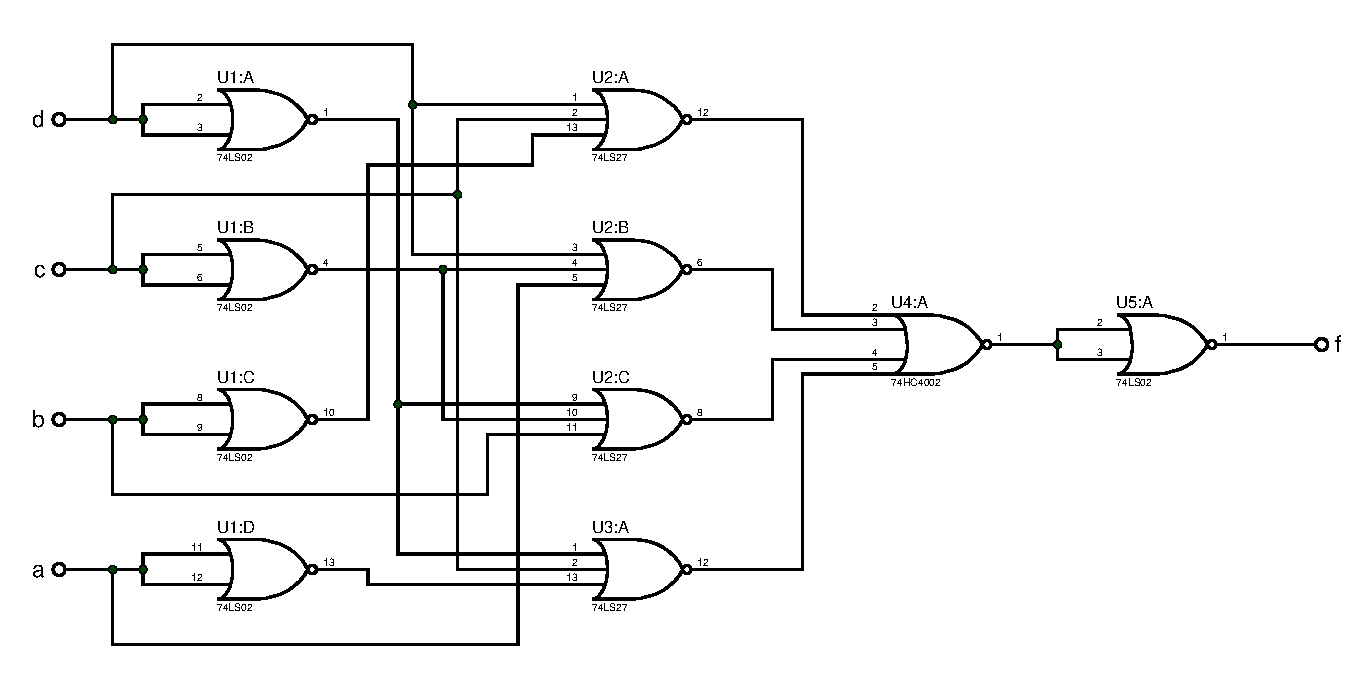
\includegraphics[width=\textwidth]{ImplementacionEj2_NOR}
    \par\end{centering}
    \caption{Circuito lógico de implementación para $f(d,c,b,a)$ - Realizado en Proteus 7.8}
\end{figure}

Para la implementación mediante el uso de sólo compuertas NOR, primero 
se debe trabajar un poco con la función obtenida aplicando las propiedades 
de De Moivre:



\end{document}